
The overall aim of parallelising the FLAME framework is to reduce the wall clock time for running a simulation. This relies on efficient parallelisation of communication and keeping the work load balanced between computing nodes. The message board library addresses the first of these and dynamic load balancing addresses the second.

To illustrate the problems in getting load balancing right, the diagram in Figure \ref{fig:load_balance_problem} shows agents on two nodes and their communication patterns. The top portion shows an unbalanced number of agents but the frequent communication is internal to each node with only occasional communication between the nodes. If agents are moved in an attempt to balance the load then frequent communication between nodes is introduced (lower portion of figure) which could mean a large increase in communication time and hence wall clock time. This example shows that measurement of communication between nodes  must be part of the load balancing algorithm as well as elapsed time for various parts of the framework.

\begin{figure}[h]
 \centering
  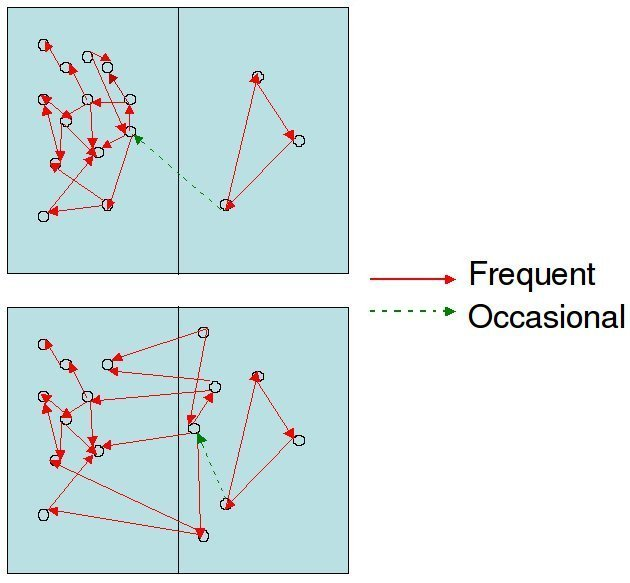
\includegraphics[scale=0.50]{load_balance.jpg}
 \caption{Illustrating some problems of load balancing}
 \label{fig:load_balance_problem}
\end{figure}

The dynamic load balancing library will therefore have to track data from two sources:

\begin{itemize}
 \item elapsed time for various parts of a FLAME run,
 \item data communication pattern and volume between nodes.
\end{itemize}

The timing data will show problems with computational load balance, where some nodes are idle and others working; and the communication data will show imbalance in the message flow between nodes, where some nodes send a lot of data and others very little. Timing data will also show whether it is the computation by the agents or time for communication that dominates the simulation. Attention can then be focused on improving load balance or improving communication balance as required.

An iteration of the model in FLAME proceeds in stages as agents move from one state to the next, therefore it will be necessary to look at data from each stage as well as the overall data for one iteration. If there is always an imbalance in load or communication for the same subset of nodes for all stages then it is easy to say that redistributing agents is necessary. However if the imbalance shows up for different nodes at different stages then the strategy for load balancing is more difficult to decide upon. 

Agents within FLAME are allowed to have dynamic memory variables (i.e.\ their size is not determined when the model is compiled but during the simulation) and so writing code to pack an agent's memory ready for transfer to another node is very difficult and execution of that code will be a large overhead in the execution of the model. As a consequence it is not envisaged that agents will be moved at every stage of an iteration. The dynamic load balancing framework will monitor the imbalances and will only decide to move agents if an imbalance is ``too great''. Experiments with the EURACE models will help determine what is meant by ``too great'' and what strategies can be adopted when seeking to achieve the best distribution of agents.

Since agents do not communicate directly with other agents but via message boards, the communication data will be the volume of message data sent from one node to another. This does not allow for identification of individual agents that may be causing problems but, by analysing the messages that are sent by a certain type of agent at the time of the imbalance it may be possible to identify a set of agents of a certain type whose redistribution could help.

Implementation has started with a timer which allows developers to insert timing into any section of FLAME, from the framework itself to the user's model functions. The details of the implementation are described in the next section. 

This timer package has proved extremely useful during analysis of the model during its development, allowing STFC to place timers around calls to all agent functions and messageboard synchronisations. The elapsed time for each function and synchronisation for each iteration can then be printed and the analysis of the top 10 longest elapsed times over the whole simulation performed. The timers are implemented to work correctly for parallel applications so that timings of each function on each process can be recorded and analysed to look for load imbalances.

